\section{Principes généraux du \textit{deep learning} liés au TAL}

L'apprentissage profond, ou \textit{deep learning}, est une sous-catégorie de ce que l'on appelle l'apprentissage machine. L'apprentissage machine est une branche des mathématiques et de l'informatique. Lors de la consommation de données, que l'on appelle entraînement, les algorithmes de ce domaine, par le biais des outils qui les implémentent, apprennent des motifs mathématiques permettant l'analyse ou la création de nouveaux contenus. L'apprentissage machine est fondé principalement sur l'algèbre linéaire, branche des mathématiques qui concernent les matrices et les vecteurs\footnote{Les matrices sont des arrangements de nombres dont la forme la plus simple à décrire serait un tableau: ainsi, un tableau [[0 1] [2 3]] comprenant 2x2 entrées est une matrice à deux dimensions. Un vecteur est un cas particulier de matrice unidimensionnelle.}. Il existe plusieurs types de tâches, mais, en traitement automatique des langues, deux ont une place plus importante que les autres:

\begin{itemize}
    \item \textbf{La classification} de valeurs. Il peut s'agir de chercher à annoter des mots comme entités nommées par exemple, d'annoter des caractères comme caractère de fin de mot dans le cadre de \textit{scripta continua}, ou encore de classer des phrases ou des textes comme portant sur tel sujet ou étant écrits par tel auteur.
    \item \textbf{La génération} de texte. Elle est désormais commune dans la traduction automatique, mais aussi dans la création de robot de discussion pour les plateformes en ligne. On distinguera les générations caractère par caractère des générations mot par mot, qui possèdent des facultés différentes: la possibilité pour l'une de trouver de nouvelles formes morphologiques, pour l'autre, l'impossibilité de proposer un mot inexistant.
\end{itemize}{}

L'apprentissage profond se distingue dans l'apprentissage machine principalement par l'absence de nécessité pour le développement d'un modèle de faire le tri manuellement parmi les données à prendre en compte statistiquement: on parle d'absence de \textit{feature extraction}. Prenons l'exemple de l'attribution d'auteur. En apprentissage machine "classique", on sélectionne entre autres l'occurrence des mots vides, l'ordre de trigramme de POS(\textit{cf.} \ref{subsec:lemma_intro})\footcite{Cafieroeaax5489}, ou encore, en poésie latine par exemple, les formations rythmiques\footcite{nagy_metre_nodate}. Au contraire, en apprentissage profond, on aura tendance à fournir le texte de manière brute ou un minimum prétraité (selon que l'on s'intéresse aux caractères plutôt qu'aux mots). C'est par exemple le procédé proposé par Ruder et al. \footcite{ruder_character-level_2016} dans une étude sur l'attribution d'auteur sur twitter: pour gérer des textes courts, avec des orthographes variées, leur proposition fut de prendre le texte brut et de traiter les caractères en brut comme données d'entraînement.

L'apprentissage machine se divise en deux autres grandes catégories, applicables à ses sous-branches: l'apprentissage supervisé et l'apprentissage non supervisé.  La différence fondamentale entre les deux protocoles réside dans la présence dans les données fournies pour l'entraînement d'étiquettes correspondant aux résultats attendus en sortie: c'est à force de voir \textit{sunt} annoté comme lemme \textit{sum} qu'il est capable de le produire de lui-même, à l'image d'un enfant à qui l'on apprend à reconnaître des animaux par exemple. En apprentissage supervisé, on peut entraîner la machine à reconnaître Molière de Corneille en lui disant: ce texte est de Corneille, ce texte est de Molière, etc.. En apprentissage non supervisé, on peut laisser la machine créer ces groupes d'elle-même, et il sera de la responsabilité de l'utilisateur d'en faire une analyse. Les apprentissages non supervisés sont principalement utilisés, en traitement automatique du langage et en apprentissage profond, pour créer des corpus: on le retrouve par exemple sur des agrégateurs tels que \textit{Google News} où les articles sont rassemblés par thème en fonction de la proximité de leur sujet. Il n'y a pas - ou peu - d'éditorialisation humaine dans ce genre de procédé. On le retrouve aussi dans les \textit{embeddings} (\textit{cf.} \ref{deep-learning:embeddings}).

En apprentissage machine, on sépare de l'entraînement l'inférence (ou prédiction): le premier permet de constituer un modèle, avec des poids (variables apprises automatiquement par celui-ci) tandis que la seconde correspond à l'utilisation de ces poids sur des données nouvelles, sans apprentissage associé par la machine (elle n'apprend plus). Durant l'entraînement, le modèle cherche à s'approcher le plus possible du résultat attendu: la différence entre les bonnes réponses et la réponse proposée est une mesure mathématique appelée \textit{loss} (perte). Cette perte est d'ailleurs transmise à l'algorithme pour affiner ses poids, et il a alors pour objectif de réduire cette dernière le plus possible. Un entraînement peut voir les données plusieurs fois: on appellera ces cycles de consultation des \textit{epochs} (époques). La répétition, encore une fois, comme avec un enfant en bas âge, permet à la machine d'enfin comprendre les motifs et à proposer les réponses attendues. 

\begin{table}[]
\centering
\begin{tabular}{lllccc}
\toprule
\multirow{2}{*}{Texte} & \multirow{2}{*}{Classe} & \multirow{2}{*}{Prédiction} & \multicolumn{3}{l}{Catégorie de classification} \\
                       &                         &                             & Corneille        & Molière       & Racine       \\ \midrule
Le Cid                 & Corneille               & Corneille                   & VP               & VN            & VN           \\
Le Misanthrope         & Molière                 & Molière                     & VN               & VP            & VN           \\
Phèdre                 & Racine                  & Racine                      & VN               & VN            & VP           \\
L'Avare                & Molière                 & Racine                      & VN               & FN            & FP          \\ \bottomrule
\end{tabular}
\caption{Exemple de classification avec les catégories afférentes. VP = Vrai Positif, FP = Faux Positif, VN = Vrai Négatif, FN = Faux Négatif}
\label{deep-learning:table:true-positives}
\end{table}

Pour mesurer l'efficacité d'un modèle supervisé, on le teste. Pour cela, on coupe généralement un corpus de données entre des données d'entraînement (\textit{train data}) et de test (\textit{test data}). On compare ensuite chacune des prédictions du modèle obtenu avec les étiquettes données dans le corpus, que l'on appelle vérité de terrain (\textit{ground truth}). Les étiquettes sont regroupées en classes: par exemple, dans le cas de Molière et Corneille, nous avons deux classes, et si nous avons 128 textes, nous avons 128 étiquettes réparties entre ces deux classes. Les résultats sont regroupés ensuite dans 4 catégories (\textit{cf.} \ref{deep-learning:table:true-positives}): les vrais positifs (VP/TP, bonne étiquette), faux positifs (FN, mauvaise étiquette pour la classe actuelle), vrais négatifs (VN/TN, reconnu comme n'étant pas de cette étiquette), faux négatif (FN, étiquette de la classe actuelle non reconnue); si toutes les étiquettes sont dans les catégories qualifiées de vraies, le modèle n'a fait aucune erreur. Ces écarts à la vérité sont mesurés principalement par 4 formules:
\begin{itemize}
    \item L'\textit{accuracy}\footnote{Le choix a été fait de ne jamais traduire \textit{accuracy} en raison de sa traduction en "précision" qui crée la confusion avec l'autre mesure \textit{precision}} mesure le nombre de vrais positifs sur le nombre total d'éléments annotés, et on pourrait le ramener à un pourcentage classique de bonne réponse. En machine learning, on le définit aussi par la formule correspondante $accuracy = \frac{VP + VN}{VP + VN + FP + FN}$
    \item La \textit{precision} mesure le pourcentage de bonnes réponses par classe sur l'ensemble des attributions effectuées sur cette classe. Elle favorise les attributions correctes à une classe sans prendre en compte les non-attributions. Sa formule est $precision = \frac{VP}{VP + FP}$
    \item Le \textit{recall} (rappel) mesure le pourcentage de réponses correctes sur l'ensemble de la classe. Elle favorise la reconnaissance de chacune des classes plutôt que les mauvaises attributions. Sa formule est $recall = \frac{VP}{VP+FN}$.
    \item Le F-Score (qui peut se découper en F1-, F2-, etc.) est la moyenne harmonique de la précision et du rappel, offrant ainsi une mesure intermédiaire. Sa formule est $F1 = \frac{2 \cdot precision\cdot recall}{precision+ recall}$
\end{itemize}{}

Par ailleurs, ces mesures permettent non seulement de mesurer l'efficacité d'un modèle, mais appliquées à des corpus de tests, elles permettent aussi de mesurer sa surspécialisation\label{deep-learning:overfitting} (\textit{overfitting}) au corpus d'entraînement. La surspécialisation correspond, à cause d'un corpus entraînement ou d'une architecture de modèle, à une incapacité du modèle de faire des prédictions en dehors de ce corpus d'origine. Sans que cela soit toujours le cas, une \textit{accuracy} à 100\% sur un corpus d'entraînement ou une loss de 0 est souvent l'un de ses signes. Pour éviter cela, on peut faire appel à plusieurs stratégies, non exclusives:
\begin{itemize}
    \item l'utilisation d'un corpus de développement ou d'évaluation (\textit{dev/eval corpus}). Il est vu lors de l'entraînement, mais n'est pas utilisé pour l'apprentissage: les erreurs ne sont pas individuellement transmises à l'algorithme. Cependant, sa perte, ou toute mesure sélectionnée dans ce cadre sont utilisées comme grand indicateur de fonctionnement: si le corpus d'entraînement fait 100\%, mais que le corpus de développement fait 80\%, on indiquera au modèle qu'il faut continuer à apprendre, quitte à s'éloigner des 100\%.
    \item l'utilisation, dans l'architecture du modèle, de \textit{dropout}, c'est-à-dire la suppression aléatoire d'une partie des données d'entraînement à chaque époque. En traitement automatique de la langue, il s'agit principalement de supprimer un mot par exemple. Cela correspondrait, dans une situation humaine, à donner des photographies d'animaux à trou (sans tête, sans jambes, etc.) afin que l'enfant reconnaisse les autres traits de l'animal. % glauque non ?
\end{itemize}

Enfin, on parle ici et là d'hyperparamètres d'architecture: il s'agit principalement de variables de configuration qui, pour un modèle, changent l'architecture ou sa manière de s'entraîner. L'un d'eux, très commun, est nommé \textit{learning rate}: il s'agit un nombre (principalement un décimal, de type 0.001) qui sert de pas pour corriger les erreurs du modèle. Plus il est bas, plus le modèle met de temps à apprendre; plus il est haut, plus le modèle risque de rater la bonne direction d'apprentissage. D'autres hyperparamètres concernent généralement la taille des réseaux neuronaux qui composent l'architecture. 

On retrouve en traitement automatique des langues quelques modules d'architecture très communs que l'on se propose d'expliquer, en partie, ici. Ces modules sont très souvent combinés ensemble: il est rare de voir une architecture complètement basée sur un seul de ces éléments.

\subsection{Embeddings}
\label{deep-learning:embeddings}

En apprentissage machine, particulièrement en TAL, la première intention est de traduire les mots par un index unique numérique, permettant ainsi de faire des calculs sur ceux-là: "\textit{fortissimi sunt belgae}" et "\textit{timendi sunt belgae}" serait traduit par [1, 2, 3] et  [4, 2, 3] où la répétition de 2 et 3 correspond à la traduction similaire de \textit{sunt} et \textit{belgae}. On appelle ces valeurs de transcodage valeurs symboliques, et le résultat \textit{one-hot vector}. Les mots sont répartis sur sur une variable discrète\footnote{Une variable discrète est une variable dont on peut énumérer les valeurs (1, 2, 3, 4, etc.). par opposition à une variable continue (0.000000001, 0.000000002, etc.)}. Ce caractère discret de la variable rend très difficile l'exploitation de l'information. Pour résoudre ce problème, mathématique, on fait usage d'embeddings, qui permettent de projeter dans l'espace les relations entre les différents mots (\textit{cf.} Figure \ref{deep-learning:embeddings}). On établit une matrice de $N$ par $M$, où $N$ correspond au nombre de mots différents rencontrés (ici 4) et $M$ une dimension choisie (ici 2). La matrice d'embeddings, si l'on avait par exemple un apprentissage en vu d'une classification par sens ou d'une classification par POS, aura tendance à proposer des résultats tels que dans la figure précédente, avec un rapprochement évident pour l'être humain de \textit{timendi} et \textit{fortissimi}, mais totalement dépendant, informatiquement, du principe de distributionalité de Firth\footcite{firth_papers_1957}.

% Exemple d'encodage one hot

\begin{figure}
    \centering
    \noindent\begin{minipage}{.32\linewidth}
        \begin{equation*}
            \begin{bmatrix}
            fortissimi \\ 
            sunt \\ 
            Belgae \\ 
            timendi \\ 
            ... \\ 
            ... \\ 
            ... \\ 
            \end{bmatrix}
            \rightarrow \begin{bmatrix}
            1 \\ 
            2 \\ 
            3 \\ 
            4 \\ 
            ... \\ 
            ... \\ 
            n \\ 
            \end{bmatrix}
        \end{equation*}
    \end{minipage}%
    \begin{minipage}{.32\linewidth}
        \begin{equation*}
            \begin{matrix}
            \textrm{Fortissimi sunt Belgae}\\ 
            \textrm{Timendi sunt Belgae}
            \end{matrix}
            \rightarrow
            \begin{matrix}
            \left [ 1\;  2\;  3 \right ]\\ 
            \left [ 4\;  2\;  3 \right ]
            \end{matrix}
        \end{equation*}
    \end{minipage}
    \caption{Exemple d'encodage\textit{ one-hot}. On constitue d'abord un dictionnaire de transcodage, puis on traduit à l'aide de celui-ci les phrases}
    \label{deep-learning:one-hot-encoding}
\end{figure}

\begin{figure}[h]
    \centering
    \noindent\begin{minipage}{.32\linewidth}
        \begin{equation*}
            \begin{matrix}
            Fortissimi \\ 
            sunt \\ 
            Belgae \\ 
            timendi \\ 
            ... \\ 
            ... \\ 
            ... \\ 
            \end{matrix}
            \rightarrow 
            \begin{bmatrix}
            0.97 & 0.85 \\ 
            0.12 & 0.85 \\ 
            0.54 & 0.28 \\ 
            0.92 & 0.90 \\ 
            ... & ... \\ 
            ... & ... \\ 
            n & ... \\ 
            \end{bmatrix}
        \end{equation*}
    \end{minipage}%
    \begin{minipage}{.32\linewidth}
        \begin{equation*}
            \begin{matrix}
                \textrm{Fortissimi sunt} \\ 
                \textrm{Belgae} \\ \\
                \textrm{Timendi sunt} \\
                \textrm{Belgae}
            \end{matrix}
            \rightarrow
            \begin{matrix}
            
            \begin{bmatrix}
            0.97 & 0.85 \\ 
            0.12 & 0.85 \\ 
            0.54 & 0.28 \\ 
            \end{bmatrix} \\ \\
            
            \begin{bmatrix}
            0.92 & 0.90 \\
            0.12 & 0.85 \\ 
            0.54 & 0.28 \\ 
            \end{bmatrix}
            
            \end{matrix}
        \end{equation*}
    \end{minipage}
    \caption{Remplacement de l'encodage one-hot par une couche  embedding. La proximité entre les vecteurs de \textit{Fortissimi} et \textit{Timendi} et la répétition des deux autres mots produisent deux phrases très proches mathématiquement.}
    \label{figure:deep-learning:embeddings-encoding}
\end{figure}

Bien sûr, ces dimensions sont d'ordinaire beaucoup plus grandes que dans l'exemple construit ici: David Bamman, lors de la création d'une telle matrice sur l'ensemble des mots présents dans les livres de langue latine du site archives.org\footcite{bamman_11k_2012}, a créé une matrice de $N=2,961,867$ et de $M=100$ (100 est une dimension assez habituelle pour $M$). Les embeddings sont très rarement utilisés comme finalités: en tant que module, ils apprendront des représentations diverses du languages, selon ce que l'on cherche à étudier. Une étude de ce qu'apprend l'algorithme en fonction de la tâche est proposée par ailleurs en \ref{subsec:lemma_resultats} pour confirmer cette situation. % Mal dit

\subsection{Linéaires}

Les couches linéaires, ou couche denses, sont des réseaux neuronaux classiques interconnectés: ils prennent une matrice de taille $N...M$ et renvoient une matrice de taille $N...O$ où $M$ et $O$ sont les tailles d'entrée et de sortie de la couche linéaire. Elles sont principalement utilisées pour classer des valeurs: on les retrouve dans ce contexte en fin de réseau. Pour des tâches telles que le repérage d'entités nommées, il est très commun de retrouver en entrée de modèle un embedding, des couches plus complexes (\textit{cf.} ci-après) et en sortie une couche linéaire qui classifiera chacun des tokens en Entité nommé ou non. 

Sur la dernière dimension d'une matrice, le modèle applique une formule particulièrement simple: il s'agit d'une fonction affine, où pour chaque valeur $M_{i}$ (ici, $i$ est un index de mot de la phrase et $M$ un vecteur) et pour chaque classe de sortie notée $j$  un poids $w_{i}{j}$ existe en plus d'une constante générale appelée biais ($b_{j}$) telle que $f(X, j) = W_{j} \dot X + b_{j}$ (\textit{cf.} figure \ref{deep-learning:simple-linear}) où X est la matrice de donnée fournie (ici, une phrase). En algèbre linéraire, une multiplication de matrice A, de taille N par M, par une matrice B, de taille M par P, résulte en une matrice de taille N par P.  

\begin{figure}
    \centering
    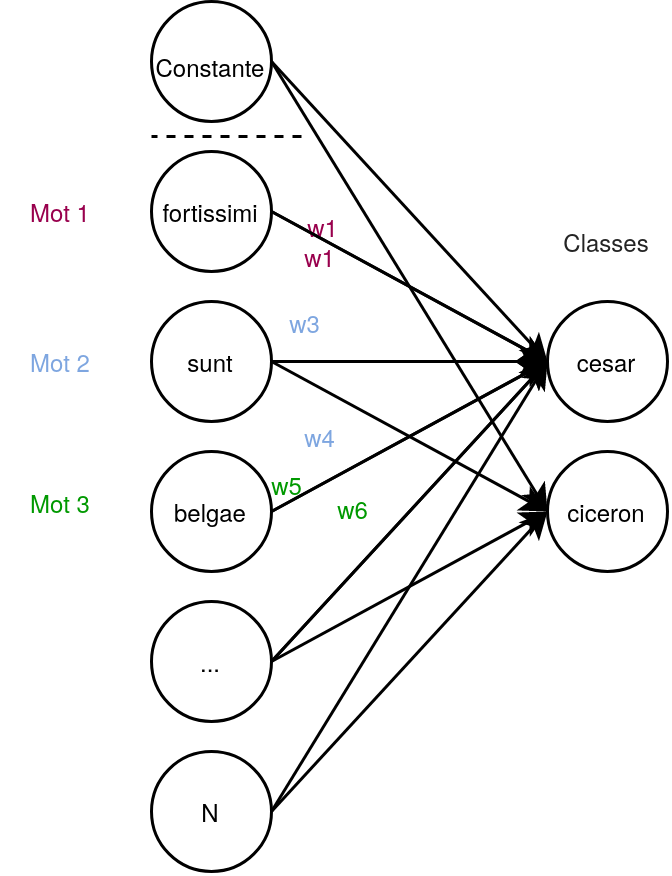
\includegraphics[width=5cm]{results/deep-learning/explanations/SimpleLinear.png}
    \caption{Exemple de couche linéaire (simplifiée)}
    \label{deep-learning:simple-linear}
\end{figure}

Par exemple, pour classer des textes par auteur, on pourrait établir un réseau neuronaux uniquement constitué de couches linéaires, qui viendraient peu à peu réduire la taille pour obtenir à la fin seulement Y valeurs de sorties, où Y est le nombre d'auteurs identifiables. Pour faire cela, sans utiliser les embeddings, nous proposons d'utiliser les fréquences de chacun des mots (fréquence de "fortissimi", "belgae", etc. dans chacun des textes). Ce réseau est appelé perceptron multi-couche (\textit{multi-layer perceptron}) et constitue le réseau neuronal le plus simple possible (\textit{cf.} figure \ref{deep-learning:mlp}). Dans une telle situation, les couches intermédiaires sont appelées \textit{hidden layers}.  Son principe de réduction des dimensions peut-être appliqué à des sorties d'autres modules avant la classification finale.

\begin{figure}
    \centering
    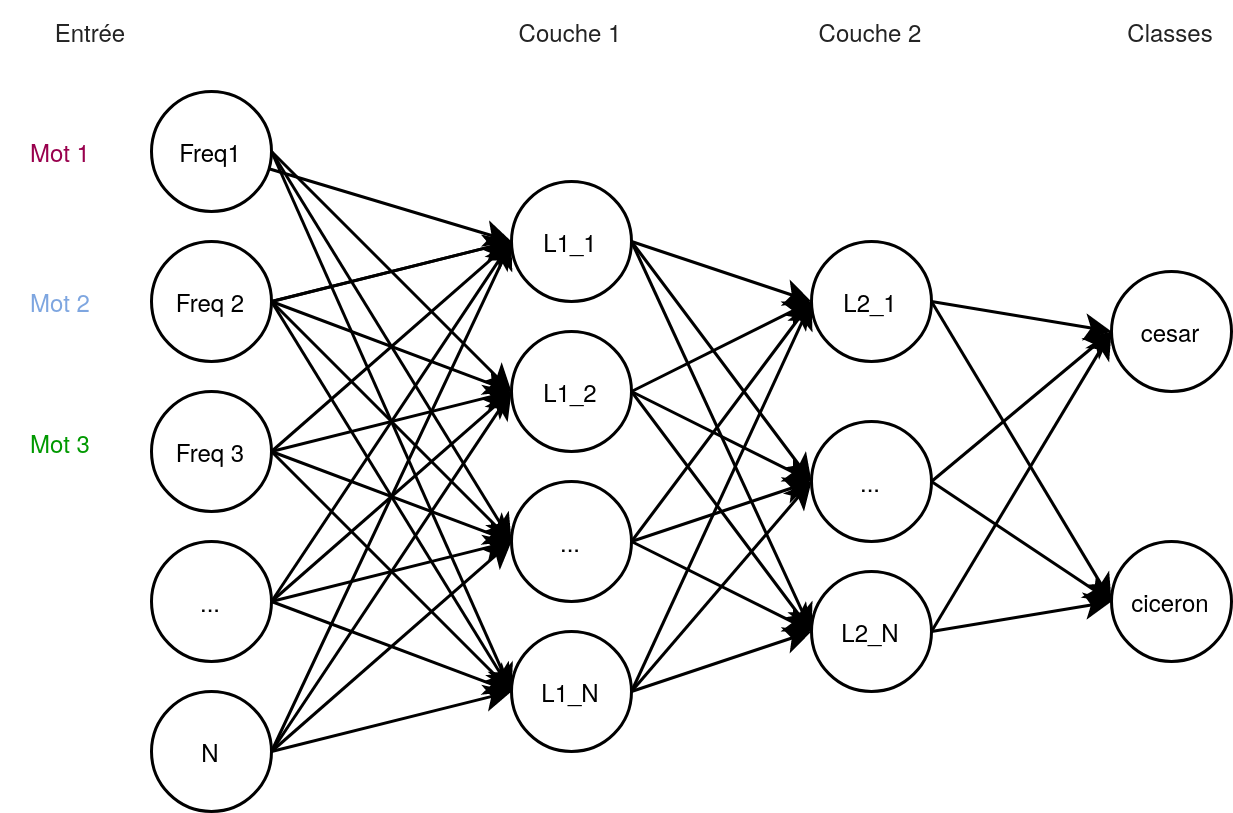
\includegraphics[width=\linewidth]{results/deep-learning/explanations/MLP.png}
    \caption{Exemple de perceptron multi-couches. Le réseau construit ici possède une entrée de taille N, une sortie de 2, et un réseau $Linear(N, L1_N) \rightarrow Linear(L1_N, L2_N) \rightarrow Linear(L2_N, 2)$}
    \label{deep-learning:mlp}
\end{figure}

\subsection{LSTM}

\subsection{CNN}